% Options for packages loaded elsewhere
\PassOptionsToPackage{unicode}{hyperref}
\PassOptionsToPackage{hyphens}{url}
\PassOptionsToPackage{dvipsnames,svgnames,x11names}{xcolor}
%
\documentclass[
  letterpaper,
  DIV=11,
  numbers=noendperiod]{scrreprt}

\usepackage{amsmath,amssymb}
\usepackage{lmodern}
\usepackage{iftex}
\ifPDFTeX
  \usepackage[T1]{fontenc}
  \usepackage[utf8]{inputenc}
  \usepackage{textcomp} % provide euro and other symbols
\else % if luatex or xetex
  \usepackage{unicode-math}
  \defaultfontfeatures{Scale=MatchLowercase}
  \defaultfontfeatures[\rmfamily]{Ligatures=TeX,Scale=1}
\fi
% Use upquote if available, for straight quotes in verbatim environments
\IfFileExists{upquote.sty}{\usepackage{upquote}}{}
\IfFileExists{microtype.sty}{% use microtype if available
  \usepackage[]{microtype}
  \UseMicrotypeSet[protrusion]{basicmath} % disable protrusion for tt fonts
}{}
\makeatletter
\@ifundefined{KOMAClassName}{% if non-KOMA class
  \IfFileExists{parskip.sty}{%
    \usepackage{parskip}
  }{% else
    \setlength{\parindent}{0pt}
    \setlength{\parskip}{6pt plus 2pt minus 1pt}}
}{% if KOMA class
  \KOMAoptions{parskip=half}}
\makeatother
\usepackage{xcolor}
\setlength{\emergencystretch}{3em} % prevent overfull lines
\setcounter{secnumdepth}{5}
% Make \paragraph and \subparagraph free-standing
\ifx\paragraph\undefined\else
  \let\oldparagraph\paragraph
  \renewcommand{\paragraph}[1]{\oldparagraph{#1}\mbox{}}
\fi
\ifx\subparagraph\undefined\else
  \let\oldsubparagraph\subparagraph
  \renewcommand{\subparagraph}[1]{\oldsubparagraph{#1}\mbox{}}
\fi

\usepackage{color}
\usepackage{fancyvrb}
\newcommand{\VerbBar}{|}
\newcommand{\VERB}{\Verb[commandchars=\\\{\}]}
\DefineVerbatimEnvironment{Highlighting}{Verbatim}{commandchars=\\\{\}}
% Add ',fontsize=\small' for more characters per line
\usepackage{framed}
\definecolor{shadecolor}{RGB}{241,243,245}
\newenvironment{Shaded}{\begin{snugshade}}{\end{snugshade}}
\newcommand{\AlertTok}[1]{\textcolor[rgb]{0.68,0.00,0.00}{#1}}
\newcommand{\AnnotationTok}[1]{\textcolor[rgb]{0.37,0.37,0.37}{#1}}
\newcommand{\AttributeTok}[1]{\textcolor[rgb]{0.40,0.45,0.13}{#1}}
\newcommand{\BaseNTok}[1]{\textcolor[rgb]{0.68,0.00,0.00}{#1}}
\newcommand{\BuiltInTok}[1]{\textcolor[rgb]{0.00,0.23,0.31}{#1}}
\newcommand{\CharTok}[1]{\textcolor[rgb]{0.13,0.47,0.30}{#1}}
\newcommand{\CommentTok}[1]{\textcolor[rgb]{0.37,0.37,0.37}{#1}}
\newcommand{\CommentVarTok}[1]{\textcolor[rgb]{0.37,0.37,0.37}{\textit{#1}}}
\newcommand{\ConstantTok}[1]{\textcolor[rgb]{0.56,0.35,0.01}{#1}}
\newcommand{\ControlFlowTok}[1]{\textcolor[rgb]{0.00,0.23,0.31}{#1}}
\newcommand{\DataTypeTok}[1]{\textcolor[rgb]{0.68,0.00,0.00}{#1}}
\newcommand{\DecValTok}[1]{\textcolor[rgb]{0.68,0.00,0.00}{#1}}
\newcommand{\DocumentationTok}[1]{\textcolor[rgb]{0.37,0.37,0.37}{\textit{#1}}}
\newcommand{\ErrorTok}[1]{\textcolor[rgb]{0.68,0.00,0.00}{#1}}
\newcommand{\ExtensionTok}[1]{\textcolor[rgb]{0.00,0.23,0.31}{#1}}
\newcommand{\FloatTok}[1]{\textcolor[rgb]{0.68,0.00,0.00}{#1}}
\newcommand{\FunctionTok}[1]{\textcolor[rgb]{0.28,0.35,0.67}{#1}}
\newcommand{\ImportTok}[1]{\textcolor[rgb]{0.00,0.46,0.62}{#1}}
\newcommand{\InformationTok}[1]{\textcolor[rgb]{0.37,0.37,0.37}{#1}}
\newcommand{\KeywordTok}[1]{\textcolor[rgb]{0.00,0.23,0.31}{#1}}
\newcommand{\NormalTok}[1]{\textcolor[rgb]{0.00,0.23,0.31}{#1}}
\newcommand{\OperatorTok}[1]{\textcolor[rgb]{0.37,0.37,0.37}{#1}}
\newcommand{\OtherTok}[1]{\textcolor[rgb]{0.00,0.23,0.31}{#1}}
\newcommand{\PreprocessorTok}[1]{\textcolor[rgb]{0.68,0.00,0.00}{#1}}
\newcommand{\RegionMarkerTok}[1]{\textcolor[rgb]{0.00,0.23,0.31}{#1}}
\newcommand{\SpecialCharTok}[1]{\textcolor[rgb]{0.37,0.37,0.37}{#1}}
\newcommand{\SpecialStringTok}[1]{\textcolor[rgb]{0.13,0.47,0.30}{#1}}
\newcommand{\StringTok}[1]{\textcolor[rgb]{0.13,0.47,0.30}{#1}}
\newcommand{\VariableTok}[1]{\textcolor[rgb]{0.07,0.07,0.07}{#1}}
\newcommand{\VerbatimStringTok}[1]{\textcolor[rgb]{0.13,0.47,0.30}{#1}}
\newcommand{\WarningTok}[1]{\textcolor[rgb]{0.37,0.37,0.37}{\textit{#1}}}

\providecommand{\tightlist}{%
  \setlength{\itemsep}{0pt}\setlength{\parskip}{0pt}}\usepackage{longtable,booktabs,array}
\usepackage{calc} % for calculating minipage widths
% Correct order of tables after \paragraph or \subparagraph
\usepackage{etoolbox}
\makeatletter
\patchcmd\longtable{\par}{\if@noskipsec\mbox{}\fi\par}{}{}
\makeatother
% Allow footnotes in longtable head/foot
\IfFileExists{footnotehyper.sty}{\usepackage{footnotehyper}}{\usepackage{footnote}}
\makesavenoteenv{longtable}
\usepackage{graphicx}
\makeatletter
\def\maxwidth{\ifdim\Gin@nat@width>\linewidth\linewidth\else\Gin@nat@width\fi}
\def\maxheight{\ifdim\Gin@nat@height>\textheight\textheight\else\Gin@nat@height\fi}
\makeatother
% Scale images if necessary, so that they will not overflow the page
% margins by default, and it is still possible to overwrite the defaults
% using explicit options in \includegraphics[width, height, ...]{}
\setkeys{Gin}{width=\maxwidth,height=\maxheight,keepaspectratio}
% Set default figure placement to htbp
\makeatletter
\def\fps@figure{htbp}
\makeatother
\newlength{\cslhangindent}
\setlength{\cslhangindent}{1.5em}
\newlength{\csllabelwidth}
\setlength{\csllabelwidth}{3em}
\newlength{\cslentryspacingunit} % times entry-spacing
\setlength{\cslentryspacingunit}{\parskip}
\newenvironment{CSLReferences}[2] % #1 hanging-ident, #2 entry spacing
 {% don't indent paragraphs
  \setlength{\parindent}{0pt}
  % turn on hanging indent if param 1 is 1
  \ifodd #1
  \let\oldpar\par
  \def\par{\hangindent=\cslhangindent\oldpar}
  \fi
  % set entry spacing
  \setlength{\parskip}{#2\cslentryspacingunit}
 }%
 {}
\usepackage{calc}
\newcommand{\CSLBlock}[1]{#1\hfill\break}
\newcommand{\CSLLeftMargin}[1]{\parbox[t]{\csllabelwidth}{#1}}
\newcommand{\CSLRightInline}[1]{\parbox[t]{\linewidth - \csllabelwidth}{#1}\break}
\newcommand{\CSLIndent}[1]{\hspace{\cslhangindent}#1}

\usepackage{makeidx}
\makeindex
\KOMAoption{captions}{tableheading}
\makeatletter
\@ifpackageloaded{tcolorbox}{}{\usepackage[many]{tcolorbox}}
\@ifpackageloaded{fontawesome5}{}{\usepackage{fontawesome5}}
\definecolor{quarto-callout-color}{HTML}{909090}
\definecolor{quarto-callout-note-color}{HTML}{0758E5}
\definecolor{quarto-callout-important-color}{HTML}{CC1914}
\definecolor{quarto-callout-warning-color}{HTML}{EB9113}
\definecolor{quarto-callout-tip-color}{HTML}{00A047}
\definecolor{quarto-callout-caution-color}{HTML}{FC5300}
\definecolor{quarto-callout-color-frame}{HTML}{acacac}
\definecolor{quarto-callout-note-color-frame}{HTML}{4582ec}
\definecolor{quarto-callout-important-color-frame}{HTML}{d9534f}
\definecolor{quarto-callout-warning-color-frame}{HTML}{f0ad4e}
\definecolor{quarto-callout-tip-color-frame}{HTML}{02b875}
\definecolor{quarto-callout-caution-color-frame}{HTML}{fd7e14}
\makeatother
\makeatletter
\makeatother
\makeatletter
\@ifpackageloaded{bookmark}{}{\usepackage{bookmark}}
\makeatother
\makeatletter
\@ifpackageloaded{caption}{}{\usepackage{caption}}
\AtBeginDocument{%
\ifdefined\contentsname
  \renewcommand*\contentsname{Table of contents}
\else
  \newcommand\contentsname{Table of contents}
\fi
\ifdefined\listfigurename
  \renewcommand*\listfigurename{List of Figures}
\else
  \newcommand\listfigurename{List of Figures}
\fi
\ifdefined\listtablename
  \renewcommand*\listtablename{List of Tables}
\else
  \newcommand\listtablename{List of Tables}
\fi
\ifdefined\figurename
  \renewcommand*\figurename{Figure}
\else
  \newcommand\figurename{Figure}
\fi
\ifdefined\tablename
  \renewcommand*\tablename{Table}
\else
  \newcommand\tablename{Table}
\fi
}
\@ifpackageloaded{float}{}{\usepackage{float}}
\floatstyle{ruled}
\@ifundefined{c@chapter}{\newfloat{codelisting}{h}{lop}}{\newfloat{codelisting}{h}{lop}[chapter]}
\floatname{codelisting}{Listing}
\newcommand*\listoflistings{\listof{codelisting}{List of Listings}}
\makeatother
\makeatletter
\@ifpackageloaded{caption}{}{\usepackage{caption}}
\@ifpackageloaded{subcaption}{}{\usepackage{subcaption}}
\makeatother
\makeatletter
\@ifpackageloaded{tcolorbox}{}{\usepackage[many]{tcolorbox}}
\makeatother
\makeatletter
\@ifundefined{shadecolor}{\definecolor{shadecolor}{rgb}{.97, .97, .97}}
\makeatother
\makeatletter
\makeatother
\ifLuaTeX
  \usepackage{selnolig}  % disable illegal ligatures
\fi
\IfFileExists{bookmark.sty}{\usepackage{bookmark}}{\usepackage{hyperref}}
\IfFileExists{xurl.sty}{\usepackage{xurl}}{} % add URL line breaks if available
\urlstyle{same} % disable monospaced font for URLs
\hypersetup{
  pdftitle={Outil de suivi de collecte MASA},
  pdfauthor={Anaël Delorme},
  colorlinks=true,
  linkcolor={blue},
  filecolor={Maroon},
  citecolor={Blue},
  urlcolor={Blue},
  pdfcreator={LaTeX via pandoc}}

\title{Outil de suivi de collecte MASA}
\author{Anaël Delorme}
\date{23/10/2023}

\begin{document}
\maketitle
\ifdefined\Shaded\renewenvironment{Shaded}{\begin{tcolorbox}[enhanced, borderline west={3pt}{0pt}{shadecolor}, sharp corners, breakable, frame hidden, boxrule=0pt, interior hidden]}{\end{tcolorbox}}\fi

\renewcommand*\contentsname{Table of contents}
{
\hypersetup{linkcolor=}
\setcounter{tocdepth}{2}
\tableofcontents
}
\bookmarksetup{startatroot}

\hypertarget{pruxe9face}{%
\chapter*{Préface}\label{pruxe9face}}
\addcontentsline{toc}{chapter}{Préface}

Le livre présente une méthode pour créer un site de suivi d'une collecte
effectuée avec Capibara \index{Capibara}. Le suite de suivi de collecte
sera accessible via un login et un mot de passe aux acteurs de la
collecte, au SSP et en SRISE/SISE.

Exemple de site de suivi :

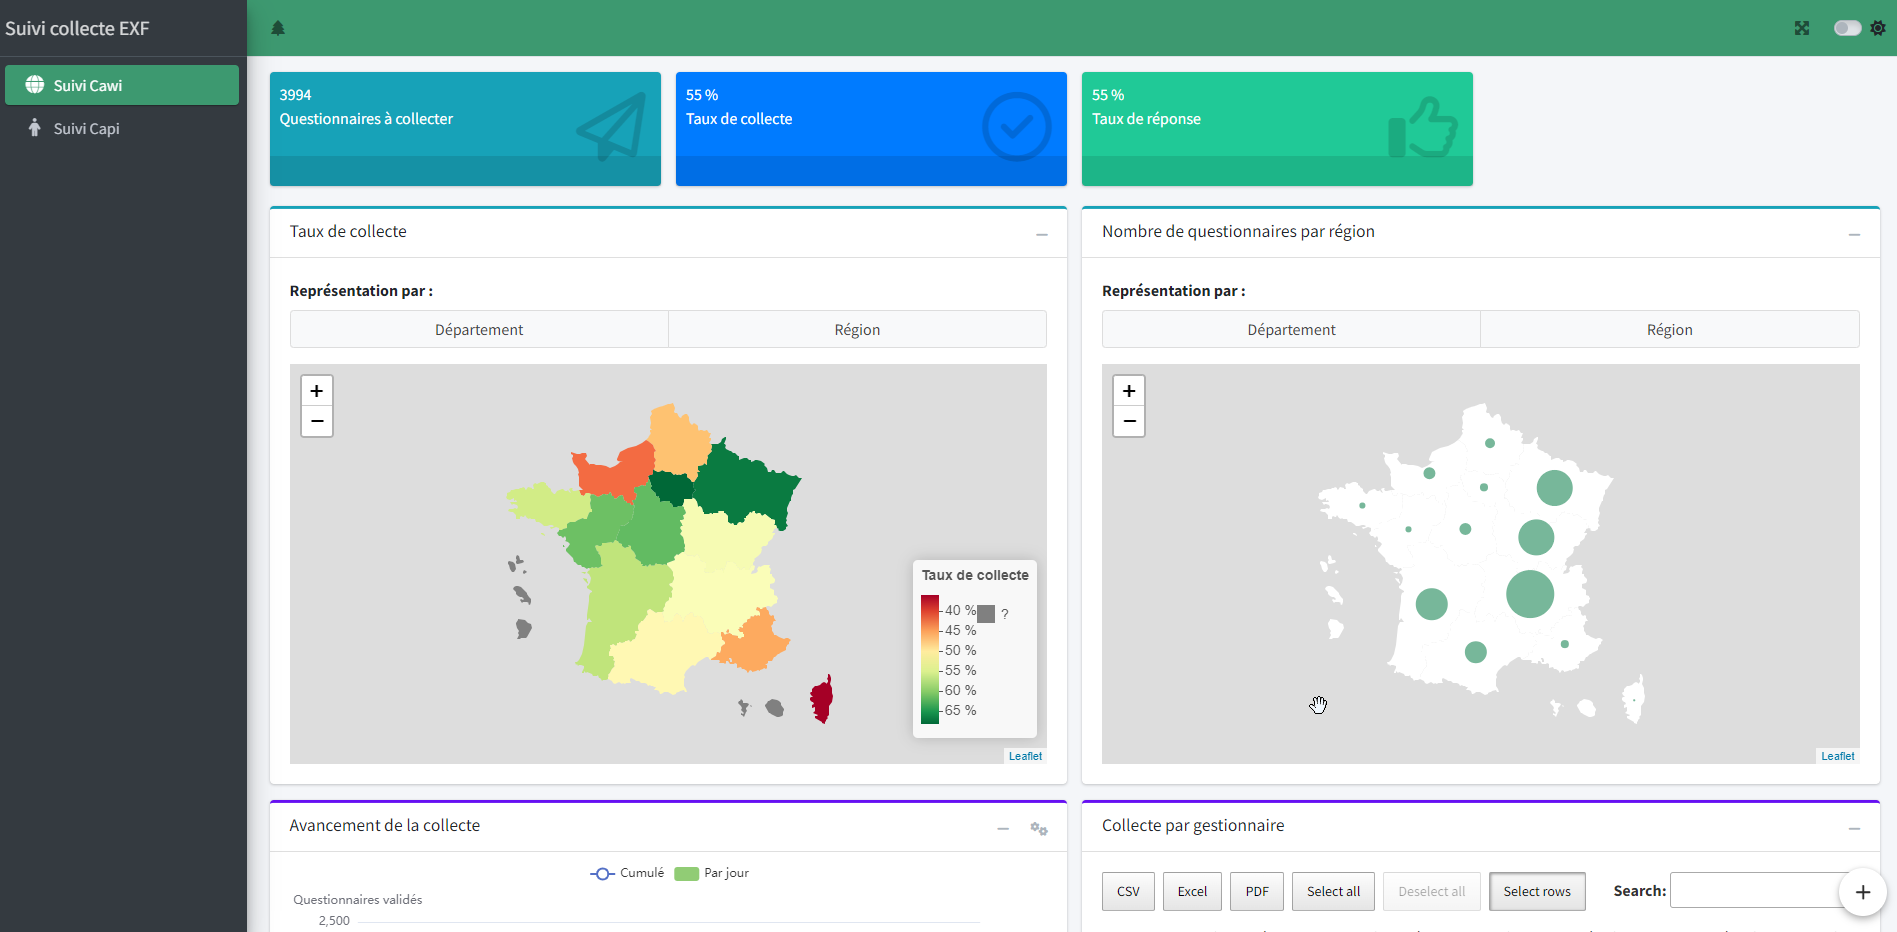
\includegraphics{./images/accueil_exf.png}

\begin{tcolorbox}[enhanced jigsaw, arc=.35mm, colbacktitle=quarto-callout-warning-color!10!white, breakable, colback=white, rightrule=.15mm, bottomrule=.15mm, coltitle=black, bottomtitle=1mm, left=2mm, opacityback=0, colframe=quarto-callout-warning-color-frame, leftrule=.75mm, toptitle=1mm, titlerule=0mm, title=\textcolor{quarto-callout-warning-color}{\faExclamationTriangle}\hspace{0.5em}{Garantie de service}, toprule=.15mm, opacitybacktitle=0.6]
La solution de suivi de collecte est basée sur un hébergement dans le
Datalab SSP Cloud. Veuillez noter qu'il n'y a aucune garantie de service
associée à cette solution. Son utilisation est basée sur la
disponibilité et les ressources actuelles, et il se peut que le service
ne soit pas toujours accessible.
\end{tcolorbox}

\bookmarksetup{startatroot}

\hypertarget{introduction}{%
\chapter{Introduction}\label{introduction}}

Les sites de suivi de collecte sont des applications internet qui
s'appuient sur les fichiers d'export de capibara pour fournir des
services utiles aux acteurs de la collecte : suivi d'avancement,
statistiques de collecte, export de listes\ldots{}

Le principe général d'architecture est assez simple :

\begin{itemize}
\tightlist
\item
  le cœur du dispositif est une application shiny, avec des packages
  additionnels pour la rendre plus efficace (bs4dash, shinywidgets,
  shinymanager\ldots),\\
\item
  cette application s'appuie sur les données exportées périodiquement
  par l'équipe SSP en charge de la collece,\\
\item
  l'application est packagée pour être déployée sur les serveurs du
  \href{https://datalab.sspcloud.fr/}{datalab SSP Cloud}.
\end{itemize}

En suivant les étapes décrites dans cette documentation, toute équipe de
collecte est capable de déployer un site de suivi.

\bookmarksetup{startatroot}

\hypertarget{pruxe9requis}{%
\chapter{Prérequis}\label{pruxe9requis}}

La création d'un site de suivi de collecte nécessite l'utilisation de
différents services gratuits. Chacun de ces services nécessite la
création d'un compte.

\hypertarget{github}{%
\section{Github}\label{github}}

(Github){[}https://github.com/{]} est un service web de stocker des
programmes informatiques et de gérer les versions de ces programmes. Les
fonctionnalités de Github qui nous intéresse pour la création des sites
de suivi de collecte :

\begin{itemize}
\tightlist
\item
  Gestion de versions : GitHub utilise Git pour permettre le suivi des
  modifications apportées aux fichiers. Vous pouvez cloner, pousser et
  tirer des référentiels Git, ce qui facilite la collaboration sur le
  code source.\\
\item
  Collaboration : GitHub permet à plusieurs contributeurs de travailler
  ensemble sur un même projet.\\
\item
  Actions GitHub; GitHub permet d'automatiser des flux de travail
  (workflows) permettant des déploiements d'application par exemple.
\end{itemize}

Pour créer un compte GitHub, suivez ces étapes :

\begin{itemize}
\tightlist
\item
  Accédez au site web de GitHub : \href{https://github.com/}{Github}
\item
  Sur la page d'accueil, vous verrez un formulaire d'inscription ``Sign
  up for Github''. Saisissez votre adresse mail pro et laissez vous
  guider.\\
\item
  Vous recevrez un e-mail de vérification à l'adresse e-mail que vous
  avez fournie. Suivez les instructions de l'e-mail pour vérifier votre
  compte.
\end{itemize}

\hypertarget{datalab-ssp-cloud}{%
\section{Datalab SSP Cloud}\label{datalab-ssp-cloud}}

Le Datalab SSP Cloud est une plateforme libre service mutualisée de
traitement de données, destinée aux statisticiens et data scientists de
l'État.

Vous pouvez vous créer un compte en allant sur la page
\href{https://datalab.sspcloud.fr/}{Datalab}, puis en haut à droit
\emph{Connexion} et \emph{Créer un compte}.

Il peut être utile de lire cette page de la documenation du datalab :
\href{https://docs.sspcloud.fr/onyxia-guide/premiere-utilisation}{Première
utilisation}

\begin{tcolorbox}[enhanced jigsaw, arc=.35mm, colbacktitle=quarto-callout-tip-color!10!white, breakable, colback=white, rightrule=.15mm, bottomrule=.15mm, coltitle=black, bottomtitle=1mm, left=2mm, opacityback=0, colframe=quarto-callout-tip-color-frame, leftrule=.75mm, toptitle=1mm, titlerule=0mm, title=\textcolor{quarto-callout-tip-color}{\faLightbulb}\hspace{0.5em}{Droits pour déposer les données}, toprule=.15mm, opacitybacktitle=0.6]
Quand votre compte est créé, contactez François Semecurbe ou Anaël
Delorme pour vous donner les droits de déposer les données.
\end{tcolorbox}

\hypertarget{jeton-daccuxe8s-personnel-github-dans-le-datalab}{%
\section{Jeton d'accès personnel Github dans le
datalab}\label{jeton-daccuxe8s-personnel-github-dans-le-datalab}}

Les programmes sont stockés sur Github et l'outil préconisé pour les
modifier est le datalab. Pour faire le lien entre les 2 outils nous
préconisons la création d'un jeton d'accès personnel côté Github, jeton
qui sera inséré dans le datalab.

\hypertarget{cruxe9ation-dun-jeton-daccuxe8s-github}{%
\subsection{Création d'un jeton d'accès
Github}\label{cruxe9ation-dun-jeton-daccuxe8s-github}}

La création d'un jeton d'accès Github est documentée par Github (en
français !) :
\href{https://docs.github.com/fr/authentication/keeping-your-account-and-data-secure/managing-your-personal-access-tokens\#cr\%C3\%A9ation-dun-personal-access-token-classic}{Création
d'un personnal access token (classic)}

\hypertarget{ajout-dans-le-datalab}{%
\subsection{Ajout dans le datalab}\label{ajout-dans-le-datalab}}

Il faut aller dans \href{https://datalab.sspcloud.fr/account}{Mon
compte} du datalab :

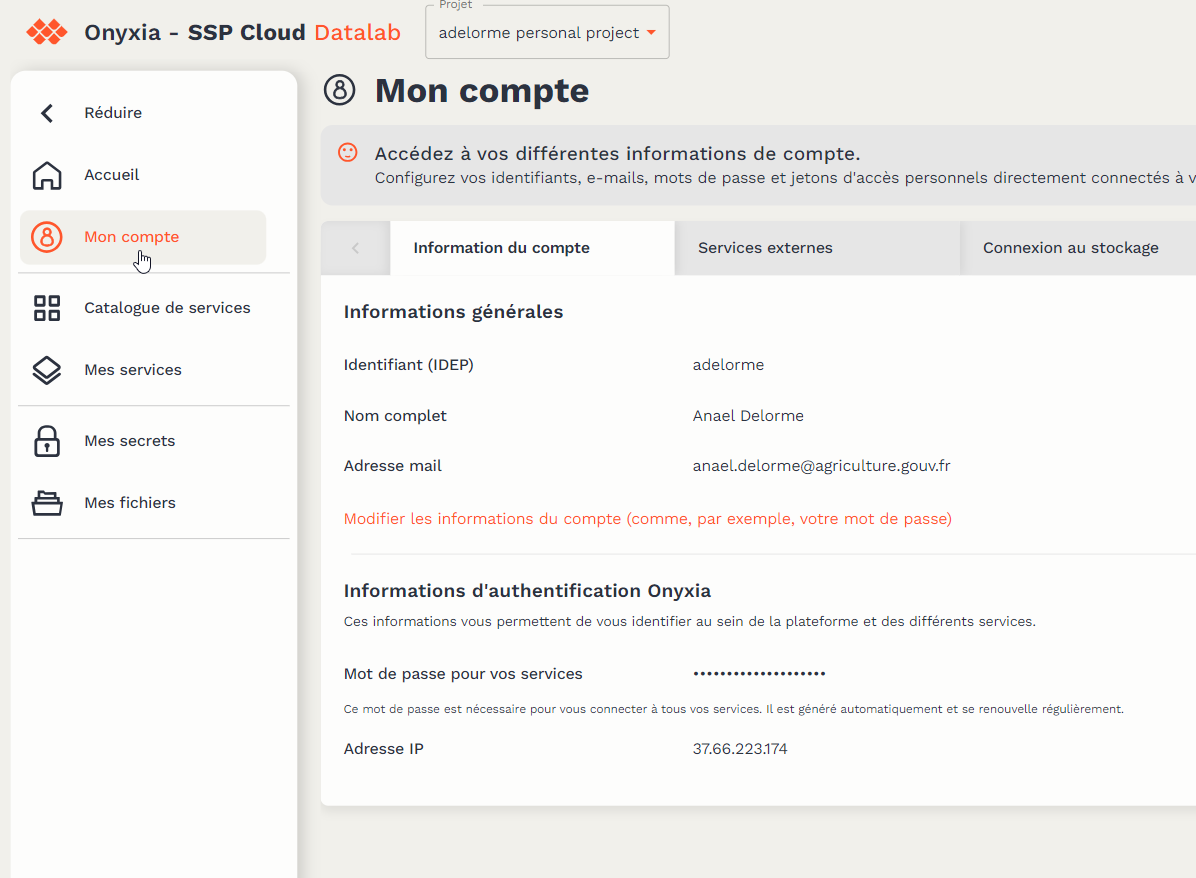
\includegraphics{./images/datalab_mon_compte.png}

Puis choisir
\href{https://datalab.sspcloud.fr/account/third-party-integration}{Service
externe} et là ajouter votre jeton Github :

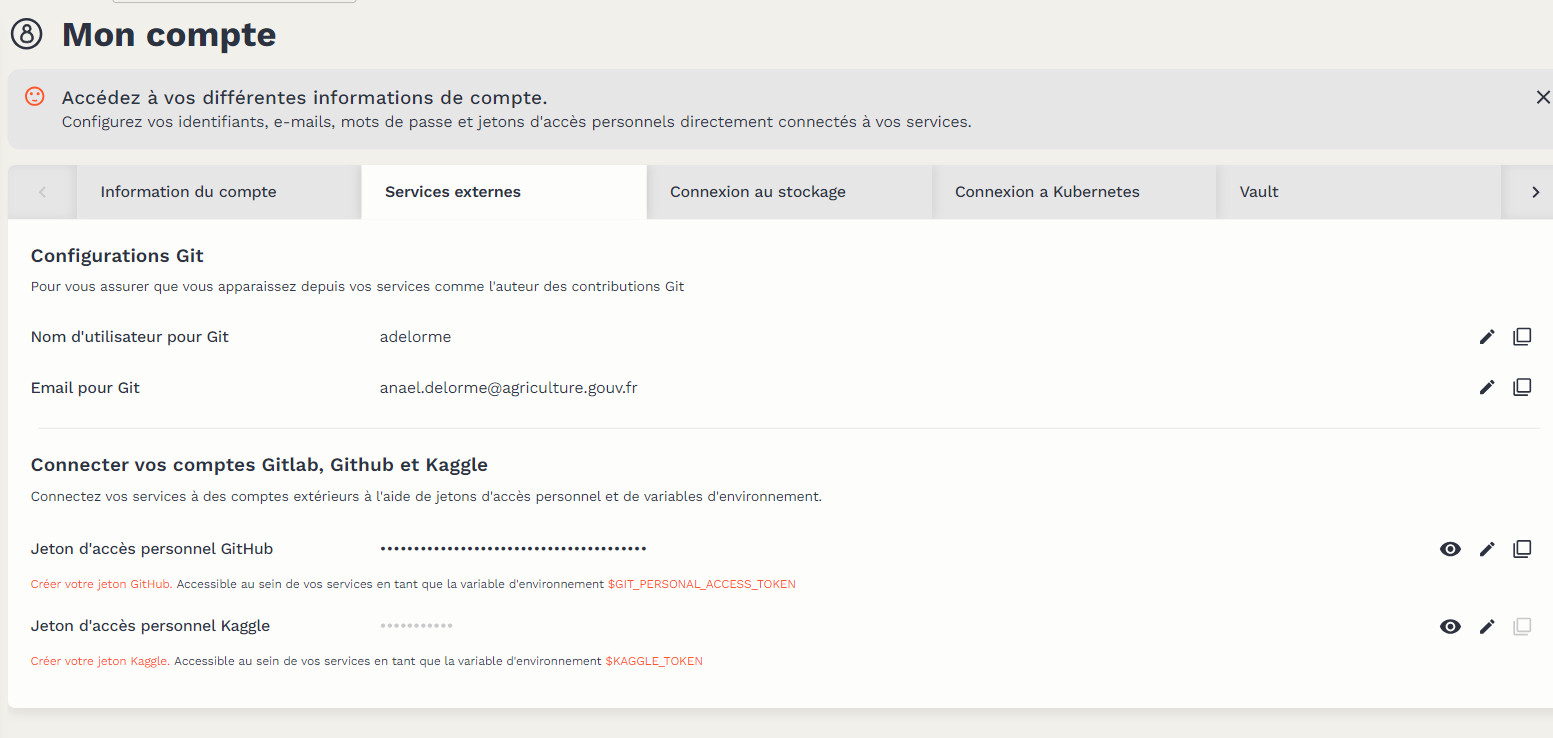
\includegraphics{./images/datalab_jeton_perso.png}

\hypertarget{dockerhub}{%
\section{DockerHub}\label{dockerhub}}

Pour déployer l'application, on a mettre l'application shiny dans un
Docker : c'est une technologie qui permet d'emballer une application ou
un logiciel, ainsi que toutes ses dépendances, dans un conteneur
virtuel. Cela permet d'assurer que l'application fonctionne de manière
fiable et de manière cohérente, quel que soit l'endroit où elle est
exécutée, que ce soit sur votre propre ordinateur, dans un centre de
données ou dans le cloud.

Le docker avec l'application shiny et ses dépendances sera stocké dans
le DockerHub : c'est une plateforme de distribution de conteneurs qui
permet aux développeurs de stocker, gérer et partager des images de
conteneurs Docker.

Pour créer un compte sur Docker Hub, suivez ces étapes :

\begin{itemize}
\tightlist
\item
  Accédez au site web de Docker Hub : \url{https://hub.docker.com}.\\
\item
  Cliquez sur le bouton ``Sign Up'' ou ``Don't have an account? Sign
  up'' pour créer un compte.\\
\item
  Suivez les étapes.\\
\item
  Vous recevrez un e-mail de vérification à l'adresse e-mail que vous
  avez fournie. Suivez les instructions de l'e-mail pour vérifier votre
  compte.
\end{itemize}

\bookmarksetup{startatroot}

\hypertarget{donnuxe9es}{%
\chapter{Données}\label{donnuxe9es}}

Les données exportées de Capibara seront déposées dans l'espace de
stockage du Datalab.

\begin{tcolorbox}[enhanced jigsaw, arc=.35mm, colbacktitle=quarto-callout-important-color!10!white, breakable, colback=white, rightrule=.15mm, bottomrule=.15mm, coltitle=black, bottomtitle=1mm, left=2mm, opacityback=0, colframe=quarto-callout-important-color-frame, leftrule=.75mm, toptitle=1mm, titlerule=0mm, title=\textcolor{quarto-callout-important-color}{\faExclamation}\hspace{0.5em}{Utilisation de données non sensibles}, toprule=.15mm, opacitybacktitle=0.6]
``Conformément aux \href{https://www.sspcloud.fr/tos_fr.md}{conditions
d'utilisation}, seules des données de type open data ou ne présentant
aucune sensibilité peuvent être stockées sur le Datalab. Le fait qu'un
fichier ait un statut de diffusion''privé'' ne suffit pas à garantir une
parfaite confidentialité.''
\end{tcolorbox}

Les données devront donc être préparées avant d'être déposées sur le
datalab.

\hypertarget{pruxe9paration-des-donnuxe9es}{%
\section{Préparation des données}\label{pruxe9paration-des-donnuxe9es}}

Toutes données permettant d'identifier une entreprise ou une personne
seront supprimées avant de remonter les données. Le format préconisé est
le parquet. Voici un exemple de code :

\begin{Shaded}
\begin{Highlighting}[]
\FunctionTok{library}\NormalTok{(tidyverse)}
\FunctionTok{library}\NormalTok{(arrow)}

\NormalTok{dossier }\OtherTok{\textless{}{-}} \FunctionTok{read.csv2}\NormalTok{(}\StringTok{"dossier.csv"}\NormalTok{)}
\NormalTok{annee\_courante }\OtherTok{\textless{}{-}} \FunctionTok{read.csv2}\NormalTok{(}\StringTok{"annee\_courante.csv"}\NormalTok{)}
\NormalTok{entreprise }\OtherTok{\textless{}{-}} \FunctionTok{read.csv2}\NormalTok{(}\StringTok{"entreprise.csv"}\NormalTok{)}
\NormalTok{gestion }\OtherTok{\textless{}{-}} \FunctionTok{read.csv2}\NormalTok{(}\StringTok{"gestion.csv"}\NormalTok{)}

\FunctionTok{write\_parquet}\NormalTok{(}\AttributeTok{x =}\NormalTok{ dossier, }\AttributeTok{sink =} \StringTok{"dossier.parquet"}\NormalTok{)}

\NormalTok{annee\_courante\_light }\OtherTok{\textless{}{-}}\NormalTok{ annee\_courante }\SpecialCharTok{\%\textgreater{}\%}
  \FunctionTok{select}\NormalTok{(Identifiant\_dossier, NOM\_DOSSIER, MAJC)}

\FunctionTok{write\_parquet}\NormalTok{(}\AttributeTok{x =}\NormalTok{ annee\_courante\_light, }\AttributeTok{sink =} \StringTok{".parquet"}\NormalTok{)}

\NormalTok{entreprise\_light }\OtherTok{\textless{}{-}}\NormalTok{ entreprise }\SpecialCharTok{\%\textgreater{}\%}
  \FunctionTok{select}\NormalTok{(}
\NormalTok{    Identifiant\_dossier,}
\NormalTok{    NOM\_DOSSIER,}
\NormalTok{    HEX\_CODE\_POSTAL\_AFFI,}
\NormalTok{    HEX\_DEPSIEGE\_AFFI,}
\NormalTok{    HEX\_REGSIEGE\_AFFI}
\NormalTok{  )}

\FunctionTok{write\_parquet}\NormalTok{(}\AttributeTok{x =}\NormalTok{ entreprise\_light, }\AttributeTok{sink =} \StringTok{"entreprise.parquet"}\NormalTok{)}

\NormalTok{gestion }\OtherTok{\textless{}{-}}\NormalTok{ gestion }\SpecialCharTok{\%\textgreater{}\%}
  \FunctionTok{select}\NormalTok{(Identifiant\_dossier, }
\NormalTok{         NOM\_DOSSIER, }
\NormalTok{         ACCEPT)}

\FunctionTok{write\_parquet}\NormalTok{(}\AttributeTok{x =}\NormalTok{ gestion, }\AttributeTok{sink =} \StringTok{"gestion.parquet"}\NormalTok{)}
\end{Highlighting}
\end{Shaded}

\hypertarget{duxe9puxf4ts-des-donnuxe9es-sur-le-datalab}{%
\section{Dépôts des données sur le
datalab}\label{duxe9puxf4ts-des-donnuxe9es-sur-le-datalab}}

Quand les données sont prépararées, il faut les déposer sur le datalab.
Le datalab offre une fonctionnalité de stockage des données (s3). Pour y
accéder, il faut aller sur le
\href{https://datalab.sspcloud.fr/}{datalab} :

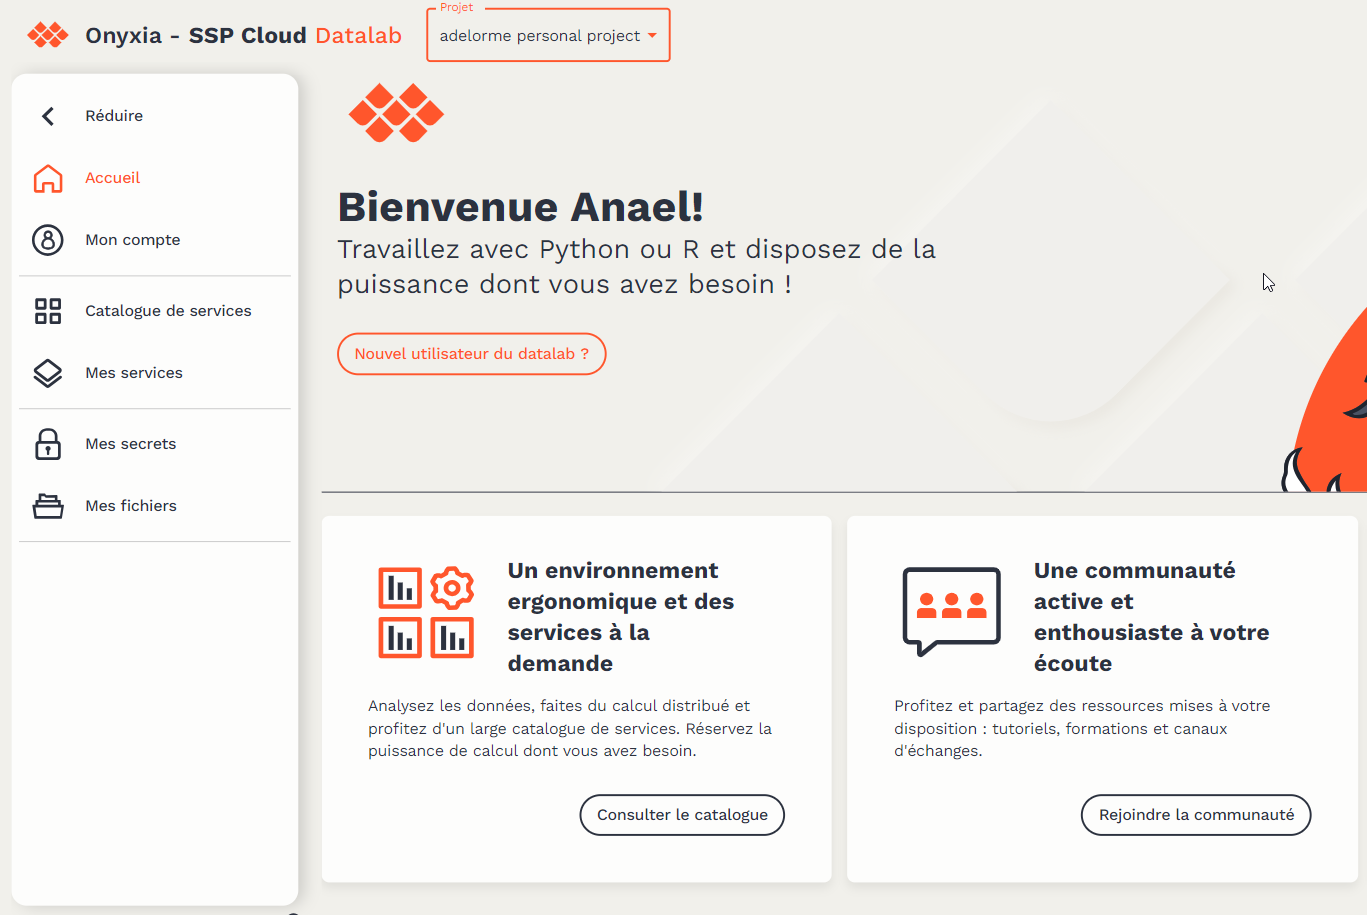
\includegraphics{./images/data_accueil_datalab.png}

Puis on choisit \emph{Mes fichiers} dans le menu de gauche :

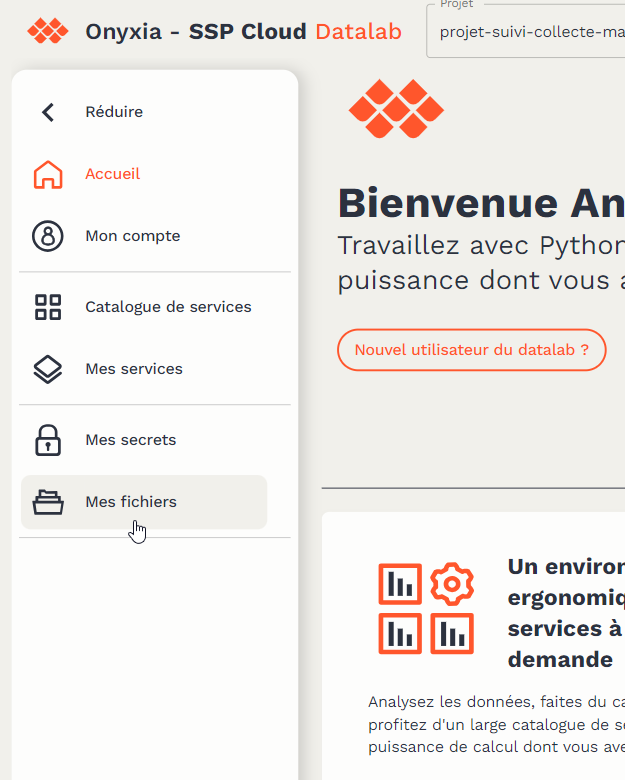
\includegraphics{./images/data_clic_mes_fichiers.png}

Là on arrive par défaut sur son lieu de stockage individuel. Pour le
site de suivi de la collecte, nous proposons d'utiliser un répertoire
(un \emph{bucket} en langage s3) partagé. Pour cela il faut choisir en
haut le projet \emph{projet\_suivi\_collecte\_masa} :

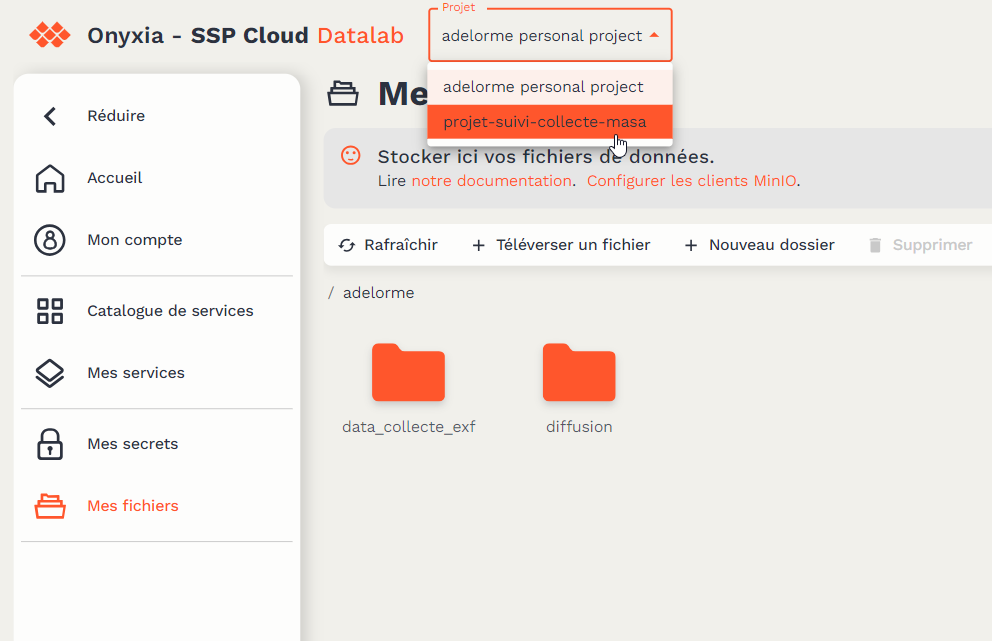
\includegraphics{./images/data_choix_projet.png}

Il ne reste plus qu'à créer un répertoire pour son site de collecte :

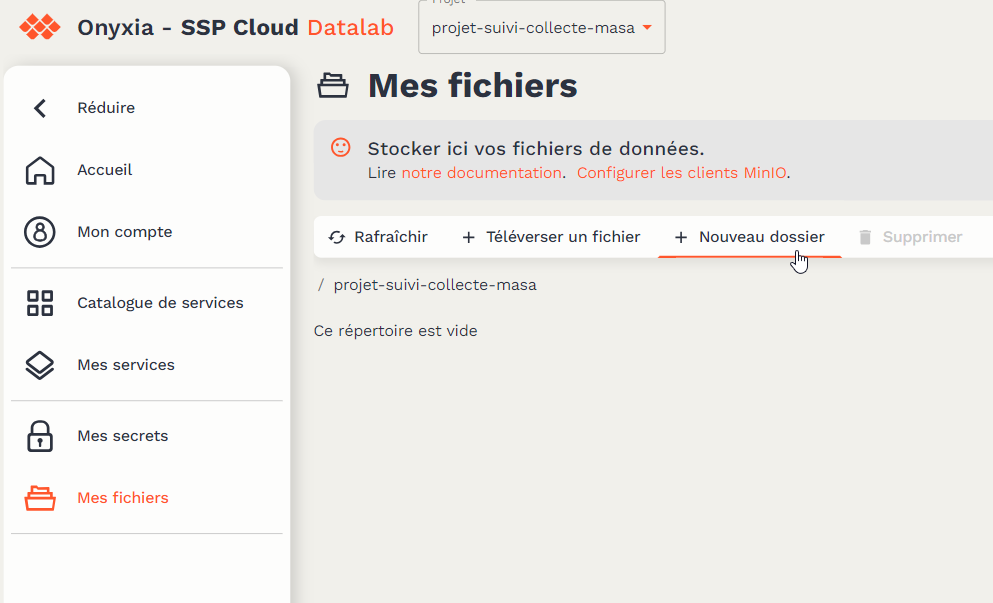
\includegraphics{./images/data_creation_nouveau_dossier.png}

En allant dans ce répertoire, il suffit de déposer le(s) fichier(s)
parquet par glisser/déposer :

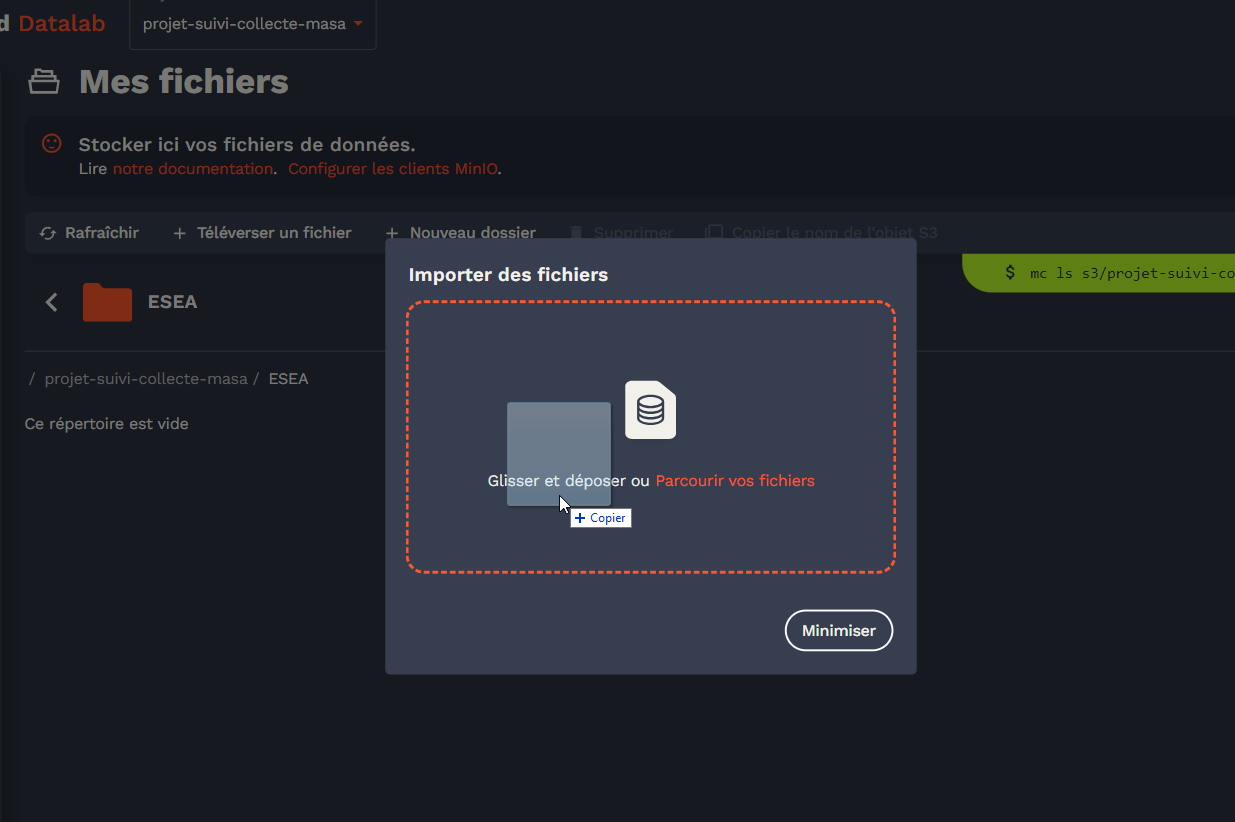
\includegraphics{./images/data_upload_data.png}

\begin{tcolorbox}[enhanced jigsaw, arc=.35mm, colbacktitle=quarto-callout-tip-color!10!white, breakable, colback=white, rightrule=.15mm, bottomrule=.15mm, coltitle=black, bottomtitle=1mm, left=2mm, opacityback=0, colframe=quarto-callout-tip-color-frame, leftrule=.75mm, toptitle=1mm, titlerule=0mm, title=\textcolor{quarto-callout-tip-color}{\faLightbulb}\hspace{0.5em}{Mise à jour des données}, toprule=.15mm, opacitybacktitle=0.6]
Régulièrement (tous les jours, toutes les semaines ?), le responsable
d'enquête mettra à jour les données. Pour cela il refera les mêmes
étapes que précédemment : export de capibara, préparation des données,
export au format parquet, téléversement dans le bucket partagé du
datalab.
\end{tcolorbox}

\bookmarksetup{startatroot}

\hypertarget{duxe9veloppement-application-shiny}{%
\chapter{Développement application
shiny}\label{duxe9veloppement-application-shiny}}

L'application de suivi de collecte est une application shiny que nous
allons déployer dans le datalab.

Pour cela nous préconisons quelques principes :

\begin{itemize}
\tightlist
\item
  utiliser le package \href{https://github.com/ThinkR-open/golem}{Golem}
  développé par Thinkr. Il encapsule l'application shiny dans un
  objectif de mise en production.\\
\item
  utiliser le datalab pour développer l'application.\\
\item
  stocker les programmes dans GitHub.
\end{itemize}

Cette partie de la documentation explique la mise en place de tout ce
qu'il faut pour développer l'application. Dans les prochaines parties
nous développerons le squelette du site de suivi, puis nous le
peuplerons avec des box.

\hypertarget{cruxe9ation-dun-repo-github}{%
\section{Création d'un repo Github}\label{cruxe9ation-dun-repo-github}}

Ce repo est le lieu de stockage des programmes du site de suivi de
collecte. La création de repo est réalisé par l'un des membres de
l'équipe avec son compte github (voir
\protect\hyperlink{pruxe9requis}{Prérequis}) :

\begin{itemize}
\tightlist
\item
  Se connecter à \href{https://github.com/}{Github}
\item
  Créer un nouveau repository
\end{itemize}

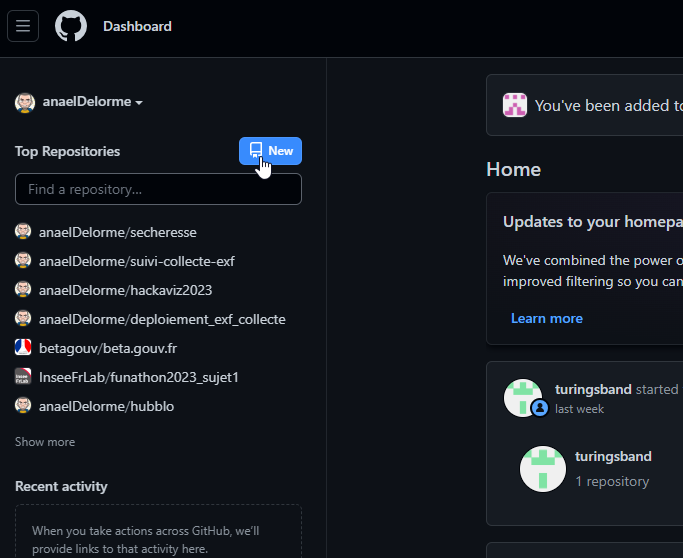
\includegraphics{./images/github_new_repository.png}

\begin{itemize}
\tightlist
\item
  saisir le nom du repo
\end{itemize}

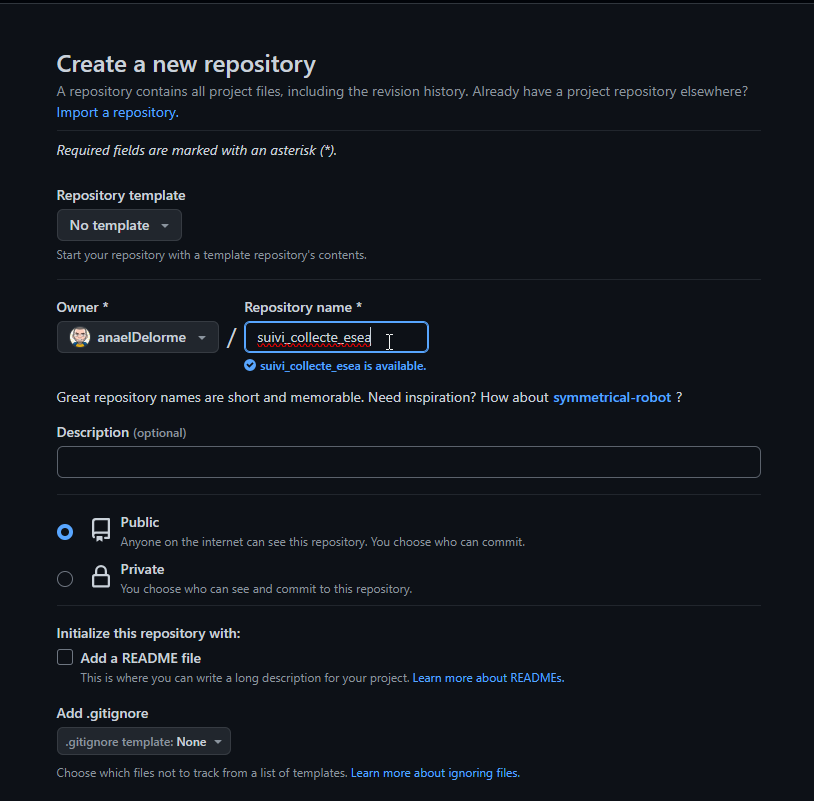
\includegraphics{./images/github_name_repository.png}

\begin{itemize}
\tightlist
\item
  laisser tout le reste tel que proposé et cliquer sur \textbf{Create
  repository}
\end{itemize}

Vous arrivez sur la page d'accueil du repo. Vous pouvez ici ajouter vos
collègues dans la rubrique \textbf{Add collaborators to this
repository}.

Avant de passer à la création du service Rstudio dans le datalab, copier
l'adresse du repo qui est disponible dans le Quick setup : dans
l'exemple ce sera
\emph{https://github.com/anaelDelorme/suivi\_collecte\_esea.git}
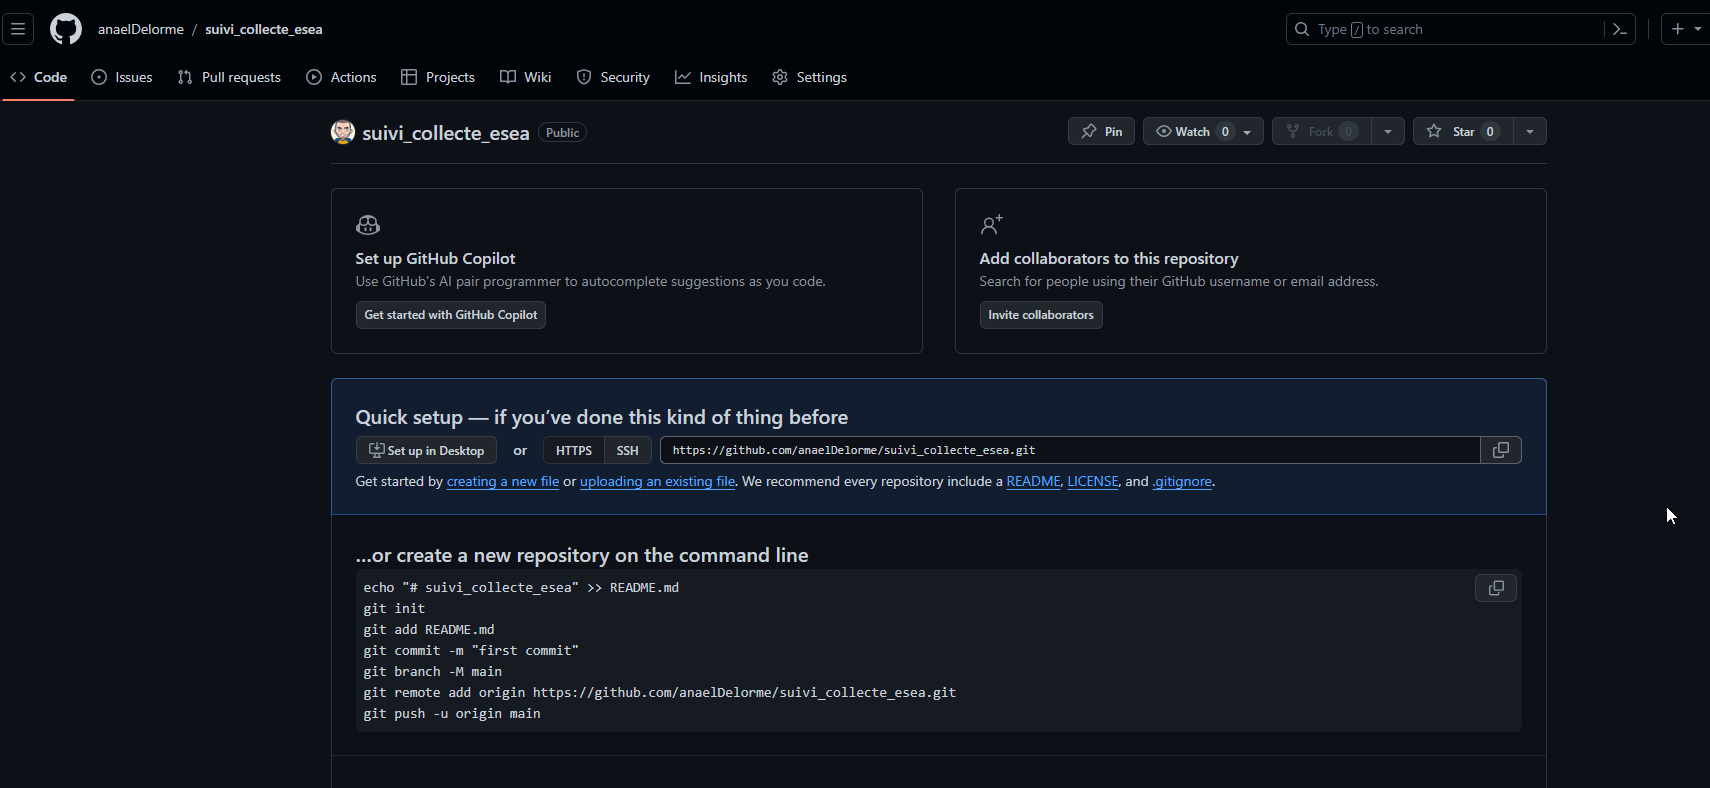
\includegraphics{./images/github_copy_link.png}

\hypertarget{cruxe9ation-dun-service-rstudio-dans-le-datalab}{%
\section{Création d'un service Rstudio dans le
datalab}\label{cruxe9ation-dun-service-rstudio-dans-le-datalab}}

Vous pourriez tout à fait travailler sur Cerise ou sur votre poste
local. Nous vous proposons de travailler sur le datalab directement :
vous avez accès à une configuration proche de celle du déploiement de
votre site.

Après vous être connecté au datalab, vous aller dans \emph{Mes
services}.

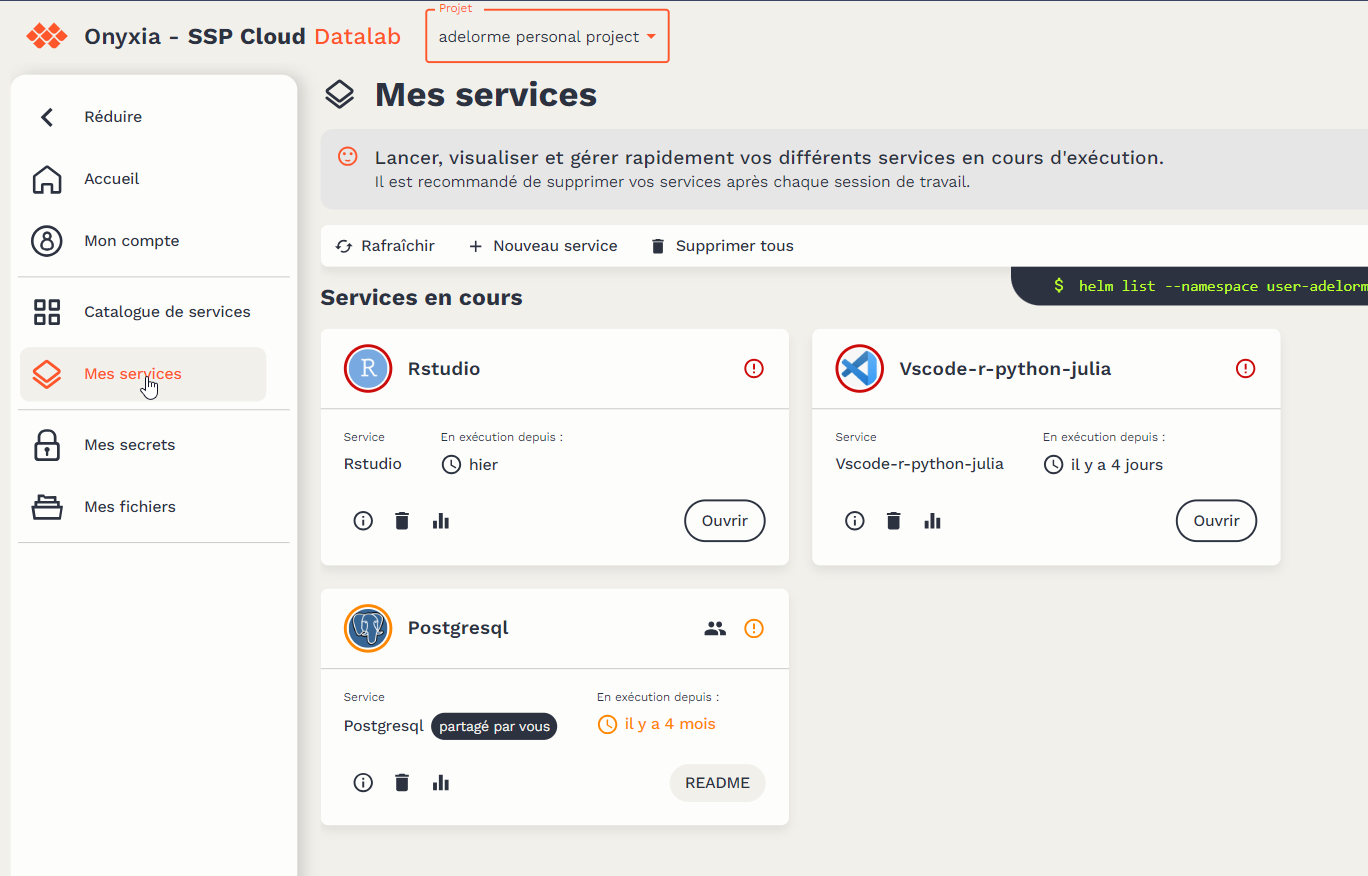
\includegraphics{./images/datalab_mes_services.png}

Puis vous cliquer sur \emph{Nouveau service} :

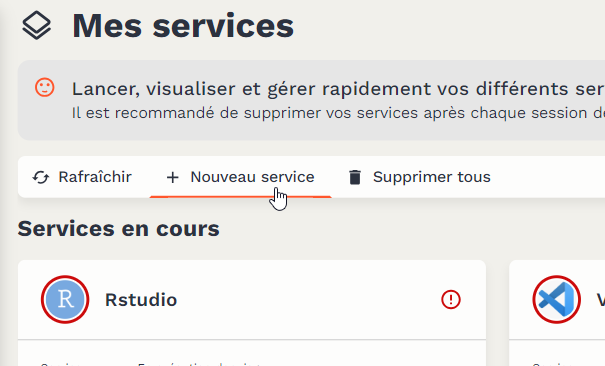
\includegraphics{./images/datalab_nouveau_service.png}

Vous allez le choix entre un Rstudio ou un Vscode-r-python-julia. Là
nous utiliserons Rstudio en cliquant sur Lancer :

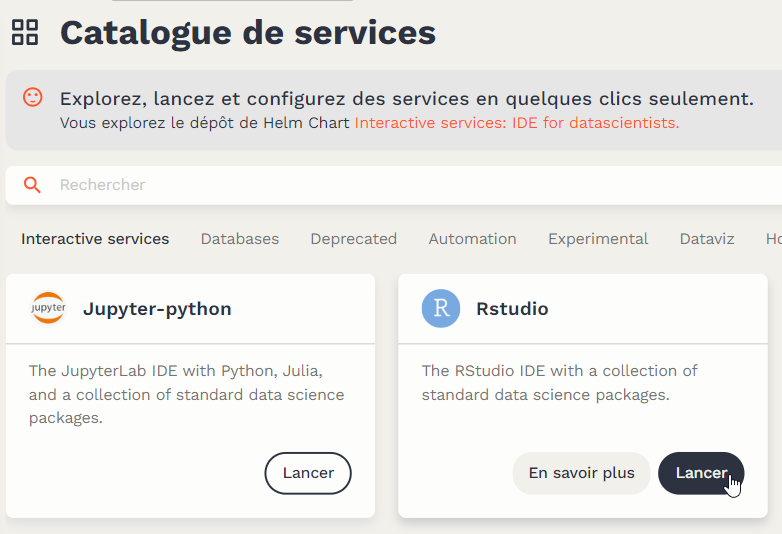
\includegraphics{./images/datalab_Rstudio_service.png}

Avant de lancer le service nous conseillons de le configurer en ouvrant
la boite \emph{Configuration Rstudio}, puis d'aller dans l'onglet
\emph{Git}. Il faut recopier dans Repository le lien du repo copier
précédemment :

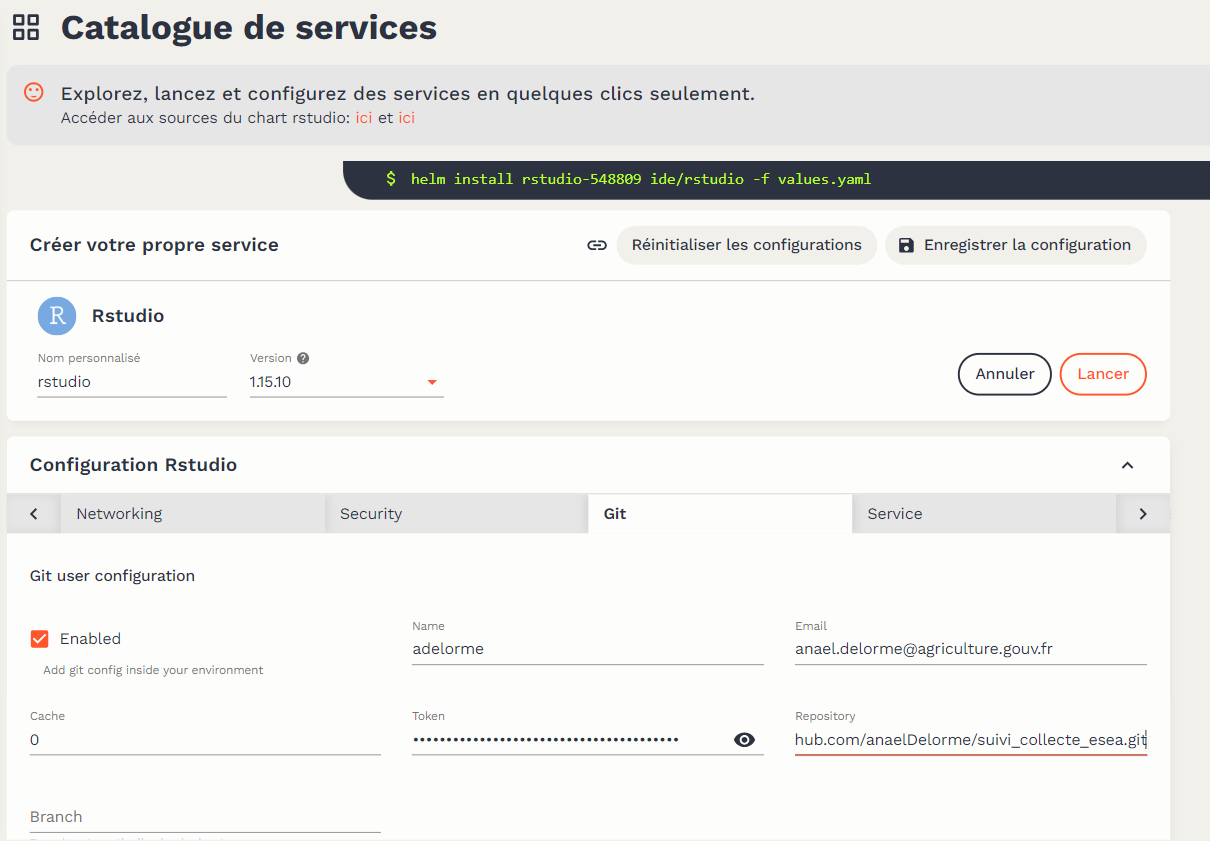
\includegraphics{./images/datalab_Rstudio_service_repo.png}

Puis clikquer sur \emph{Lancer}. Après quelques instants le service
Rstudio sera disponible et vous pourrez vous y connectant avec
l'identifiant onyxia et le mot de passe indiqué à l'écran.

Si tout s'est bien passé, vous arrivez dans un Rstudio classique avec
dans les Files un répertoire vide correspondant au répertoire du Github.

\hypertarget{installation-des-packages-utiles}{%
\section{Installation des packages
utiles}\label{installation-des-packages-utiles}}

La création d'un site de suivi de collecte nécessite l'installation de
packages. Voici la commande à lancer :

\begin{Shaded}
\begin{Highlighting}[]
\FunctionTok{install.packages}\NormalTok{(}\FunctionTok{c}\NormalTok{(}\StringTok{"tidyverse"}\NormalTok{, }\StringTok{"arrow"}\NormalTok{, }\StringTok{"shiny"}\NormalTok{, }\StringTok{"shinyWidgets"}\NormalTok{, }\StringTok{"bs4Dash"}\NormalTok{, }\StringTok{"shinymanager"}\NormalTok{, }\StringTok{"leaflet"}\NormalTok{, }\StringTok{"config"}\NormalTok{, }\StringTok{"DT"}\NormalTok{, }\StringTok{"echarts4r"}\NormalTok{, }\StringTok{"geojsonio"}\NormalTok{, }\StringTok{"glue"}\NormalTok{, }\StringTok{"golem"}\NormalTok{, }\StringTok{"htmlwidgets"}\NormalTok{, }\StringTok{"janitor"}\NormalTok{, }\StringTok{"sf"}\NormalTok{, }\StringTok{"testthat"}\NormalTok{, }\StringTok{"geojsonio"}\NormalTok{))}
\end{Highlighting}
\end{Shaded}

\hypertarget{cruxe9ation-du-projet-golem}{%
\section{Création du projet Golem}\label{cruxe9ation-du-projet-golem}}

Allez dans le répertoire créé dans votre Rstudio, puis lancer la
commande :

\begin{Shaded}
\begin{Highlighting}[]
\NormalTok{golem}\SpecialCharTok{::}\FunctionTok{create\_golem}\NormalTok{(}\AttributeTok{path =} \StringTok{"suiviCollecteESEA"}\NormalTok{, }\AttributeTok{check\_name =} \ConstantTok{TRUE}\NormalTok{, }\AttributeTok{open =} \ConstantTok{TRUE}\NormalTok{)}
\end{Highlighting}
\end{Shaded}

\bookmarksetup{startatroot}

\hypertarget{section}{%
\chapter{}\label{section}}

\bookmarksetup{startatroot}

\hypertarget{section-1}{%
\chapter{}\label{section-1}}

\bookmarksetup{startatroot}

\hypertarget{section-2}{%
\chapter{}\label{section-2}}

\bookmarksetup{startatroot}

\hypertarget{section-3}{%
\chapter{}\label{section-3}}

\bookmarksetup{startatroot}

\hypertarget{section-4}{%
\chapter{}\label{section-4}}

\bookmarksetup{startatroot}

\hypertarget{references}{%
\chapter*{References}\label{references}}
\addcontentsline{toc}{chapter}{References}

\hypertarget{refs}{}
\begin{CSLReferences}{0}{0}
\end{CSLReferences}



\printindex

\end{document}
